
\documentclass[11pt, openany]{report}
\usepackage{euler}
\usepackage{amsmath}
\usepackage[utf8]{inputenc}
\usepackage[linesnumbered,ruled,vlined]{algorithm2e}
\usepackage[OT1]{fontenc}
\usepackage[a4paper,left=2cm,right=2cm,top=2cm,bottom=2cm]{geometry}
\usepackage[frenchb]{babel}
\usepackage{libertine}
\usepackage[pdftex]{graphicx}
\usepackage{lmodern}
\usepackage{graphicx}
\usepackage{float}
\usepackage[export]{adjustbox}
\setlength{\parindent}{0cm}
\setlength{\parskip}{1ex plus 0.5ex minus 0.2ex}
\newcommand{\hsp}{\hspace{20pt}}
\newcommand{\HRule}{\rule{\linewidth}{0.5mm}}
\SetKwFor{For}{pour}{faire}{endfor}
\SetKwFor{While}{tant que}{faire}{endw}
\SetKwIF{If}{ElseIf}{Else}{si}{alors}{else si}{sinon}{endif}
\setlength{\parindent}{2em}
\setlength{\parskip}{0.2em}
\usepackage{titlesec}
\usepackage[nottoc,notlof,notlot]{tocbibind}
\titleformat{\section}{\bfseries\Large}{\thesection.}{0.5em}{}
\titleformat{\subsubsection}{}{\thesubsubsection}{1em}{\itshape}
\renewcommand\bibname{References}
\usepackage[%
	colorlinks=true,
	pdfborder={0,0,0},
	linkcolor=blue
]{hyperref}
\usepackage{fancyhdr}
\setlength{\headheight}{8pt}
\pagestyle{headings}
\renewcommand{\baselinestretch}{1}
\rfoot{Page \thepage}
\normalfont
\setlength{\parskip}{0.5em}
\begin{document}
\begin{titlepage}
  \begin{sffamily}
  \begin{center}
    % Upper part of the page. The '~' is needed because \\
    % only works if a paragraph has started.
    % \includegraphics[scale=0.04]{}~\\[1.5cm]


\begin{figure}[h!]
  \begin{minipage}{0.48\textwidth}
   \centering
  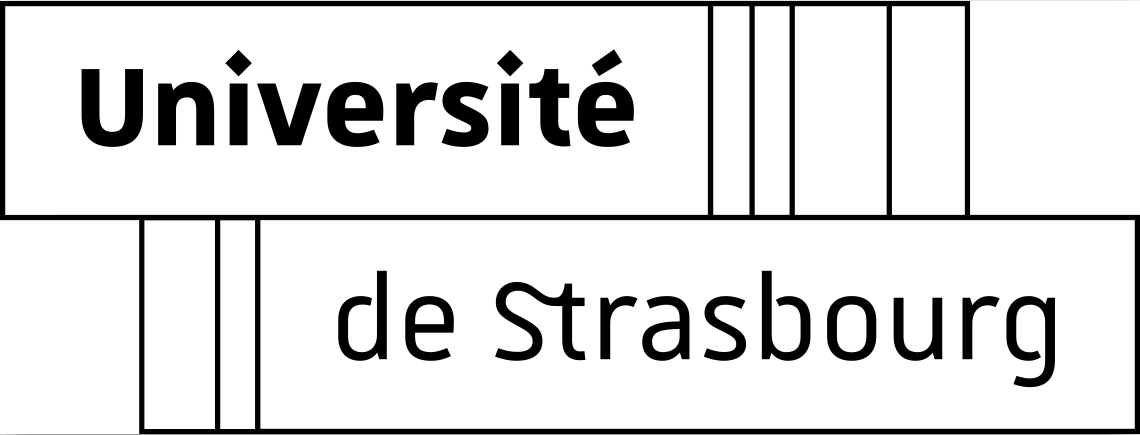
\includegraphics[width=0.6\linewidth,left]{unistra.png}
  \end{minipage}\hfill
  \begin{minipage}{0.48\textwidth}
   \centering
  
\includegraphics[width=0.6\linewidth,right]{eost.png}
  \end{minipage}
\end{figure} 


    \textsc{\LARGE \\
Université de Strasbourg}\\[3cm]

    \textsc{\Large Rapport intermédiaire de stage Master}\\[1.5cm]

    % Title
    \HRule \\[0.4cm]
    { \huge \bfseries
Développement d'un outil d'analyse automatique de longues séries temporelles de mouvements du sol et de détection d'anomalies : application à des produits issues de données satellitaires Sentinel-1 et Sentinel 2 \\[0.4cm] }

\HRule \\[2cm]
	  	
    % Author and supervisor
    \begin{minipage}{0.4\textwidth}
      \begin{flushleft} \large
      	\textsc{Etudiant :}\\ 
        \textsc{Pambou Moubogha Eddy}\\
         \textsc{année scolaire 2020-2021}\\
      \end{flushleft}
    \end{minipage}
    \begin{minipage}{0.4\textwidth}
      \begin{flushright} \large
        \textsc{Encadrant :}\\ 
        \textsc{Jean-Philippe Malet}\\
      \end{flushright}
    \end{minipage}

    \vfill

    % Bottom of the page
    {\large 3 mai 2021 — 30 septembre 2021}

  \end{center}
  \end{sffamily}
\end{titlepage}
\newpage

\chapter{Introduction}
Les glissements de terrain apparaissent lorsqu'une masse de terre descend sur un plan de glissement, provoqués par les activités anthropiques ou des phénomènes climatiques, géologiques ou géomorphologiques.
Ces déplacements peuvent être lents (quelques millimètres par an) ou rapides (quelques centaines de mètres par jour). \par

Ces mouvements peuvent être à l'origine de catastrophes naturelles causant des pertes humaines et des dommages importants sur les infrastructures. Au plan mondial, les mouvements de terrain causent chaque année la mort de 800 à 1000 personnes. En France, ce risque concerne environ 7000 communes et présente, pour un tiers d’entre elles, un niveau de gravité fort.\par

Bien que la détection de ces phénomènes soit difficile, il est possible de surveiller les mouvements du sol dans les zones sensibles en utilisant les techniques de télédétection. L'interférométrie radar et l'imagerie optique sont deux techniques de télédétection qui permettent de mésurer les mouvements du sol. L'interférométrie radar permet de mésurer la déformation du sol dans la ligne de visée du satellite avec une précision millimétrique en calculant la différence de phase entre deux acquisitions. Cependant, cette technique n'est pas adaptée pour mésurer les déplacements rapides. De plus, la déformation mésurée est une projection du vecteur déformation sur la ligne de visée du satellite, ne facilitant pas ainsi son interprétation. Contrairement à l'imagerie radar, l'imagerie optique permet de mésurer les déplacements rapides et est sensible aux composantes Nord-Sud et Est-Ouest de la déformation.

Il existe plusieurs algorithmes de correlation d'images. Des chercheurs de l'EOST travaillant au sein de l'équipe déformation active ont récemment proposé une nouvelle version de MPIC-OPT, un workflow permettant de calculer des champs de déplacement en utilisant la corrélation d'images. Cette nouvelle approche utilise la décomposition en composantes indépendantes (ICA) pour débruiter les déplacements bruts. Cependant, cette méthode statistique nécessite des heuristiques pour identifier les sources contribuant aux signaux d'interêt. Actuellement, cette étape n'est pas automatique, elle est réalisée en utilisant les connaissances géologiques de la zone d'étude.\par

Dans un premier temps, est de propose d'automatiser la détection de glissements de terrain en utilisant les techniques de machine learning. Dans un second temps, il vise à dévélopper une approche pour fusionner les données de l'imagerie radar et de l'imagerie optique afin d'avoir une meilleure cartographie des glissements de terrain.

\chapter{Présentation de l'organisme d'accueil}
L'Ecole et Observatoire des Sciences de la Terre (EOST) est une école d'ingénieurs en géophysique
créé en 1935 par Edmond Rothé. Comme son nom l'indique l'EOST est également un observatoire. L’objectif premier de l’UMS830 est de faciliter l'observation pérenne des phénomènes naturels et de rendre accessible les données recueillies à la communauté scientifique. Ses tâches d'observation entrent dans le cadre des Services Nationaux d'Observation (SNO) labellisés par l'Institut National des Sciences de l'Univers du CNRS. Au total, l'EOST est impliqué dans dix services d'observation dont il est pilote au plan national ou partenaire actif. Ils concernent le domaine "Terre solide" et le domaine "Surfaces et interfaces continentales".

Ce stage s'effectue au sein de l'équipe Déformation Active. Les travaux de l'équipe portent sur la déformation lithosphérique, le fonctionnement des failles sismiques et la déformation de sub-surface. Elle est fédérée autour de plusieurs disciplines, telles que la géodésie, la tectonique active, la géomorphologie et la paléosismologie. Elle appuie fortement sa recherche sur les données acquises par les observatoires de l'EOST gérés par ses membres et sur des chantiers régionaux, principalement situés en Méditerranée et en Afrique.

\begin{figure}[H]
  \centering
  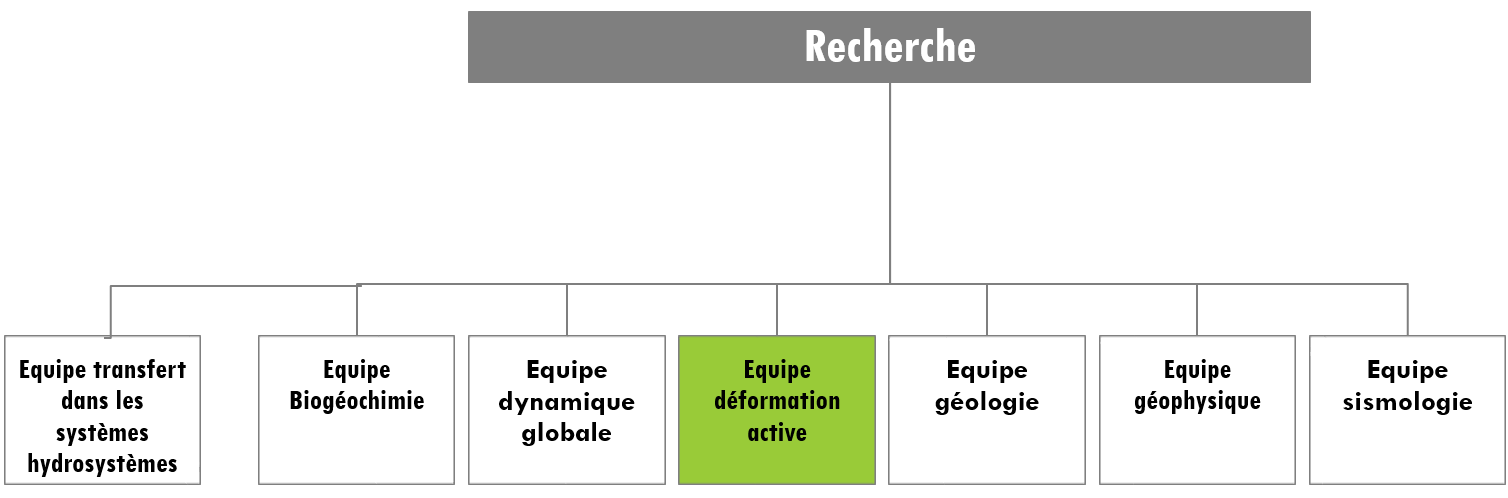
\includegraphics[width=0.6\linewidth]{recherche.png}
  \caption{Organigramme simplifié du pôle Recherche de l'EOST.}
\end{figure}

\chapter{Missions}
Ce stage est centré sur deux objectifs principaux. Le premier consiste à développer une approche pour détecter automatiquement les glissements de terrain sur les données satellitaires en utilisant une technique d'apprentissage non-supervisée. Le second vise à proposer une méthode permettant d'obtenir un champ de déplacements regroupant à la fois les déplacements calculés à partir des données de l'imagerie radar et ceux  calculées à partir des données de l'imagerie optique. Les méthodes dévéloppées doivent être testées sur les données des satellites Sentinel-1 et Sentinel-2 acquises dans les Alpes.
\section{Tâches réalisées}
De façon générale, un glissement de terrain se traduit par une série temporelle de déplacements cumulés croissante ou décroissante. Un glissement pouvant être active ou endormi, on peut observer une composante cyclique qui vient s'additionner à cette tendance.

Ma première idée a donc été d'utiliser un test statistique qui permet détecter la présence d'une tendance dans une série temporelle. Il existe plusieurs tests statistiques pour y parvenir, le plus utilisé étant le test de dickey fuller augmenté. Mon choix s'est porté sur ce dernier. Les données n'étant pas échantillonnées régulièrement, il faut les rééchantilonner avant d'appliquer le test. Mais le rééchantillonnage conduit à une perte importante du signal de départ, compliquant ainsi l'interprétation des résultats du test. 

Ma deuxième idée a été d'utiliser le test statistique de Fischer qui permet tester la significativité des coefficients d'une regression linéaire. Ce choix est motivée par le fait que certains déplacements sont bruités. Ce bruit peut se traduire par des oscillations de grandes amplitudes qui influencent les résultats de la régression. Cette méthode a donné des résultats convainquants lorsqu'une tendance linéaire est claire mais elle est moins robuste en présence du bruit. Par exemple, elle n'est pas efficace pour détecter les séries temporelles stables (déplacements nuls).

Ma troisième approche est une approche que j'ai trouvée dans la bibliographie. Elle consiste à ne sélectionner que les séries temporelles qui montrent des déplacements 
importants. Avec cette méthode, il faut estimer la vitesse moyenne de chaque déplacement par regression linéaire sur chaque composante du mouvement. Les vitesses moyennes estimées permettent ensuite de calculer la norme du vecteur vitesse. Finalement, un déplacement est considéré comme important si sa vitesse moyenne est supérieure à un certain seuil, ce  seuil étant proportionnel à l'écart-type des vitesses.

En combinant le test statistique de Fischer et le filtrage des vitesses en utilisant l'écart-type, j'ai considérablement réduit le nombre de pixels sans interêt. Après cette phase de filtrage, j'ai effectué le clustering des séries temporelles restantes à l'aide d'une méthode de clustering par densité. Contrairement à une méthode de clustering comme les k-means, les méthodes de clustering par densité ne necessitent pas un nombre prédéfini de classes et sont plus adaptées pour détecter des clusters de forme non convexe. Les deux algorithmes de clustering par densité les plus connus sont DBSCAN et HDBSCAN. J'ai choisi d'utiliser HDBSCAN car il donne de meilleurs résultats lorsque les clusters ont des tailles significativement differentes.

Puisque les séries temporelles sont géoréférencées, il est possible de visualiser les résultats du clustering sur Google Earth. Les premiers tests réalisés sur la zone Aiguilles montrent que je parviens à détecter le glissement de terrain de la Valette. Cependant cette zone comporte des glissements plus petits que ma méthode ne parvient pas à détecter (Figure 3.1).

\begin{figure}[H]
  \centering
  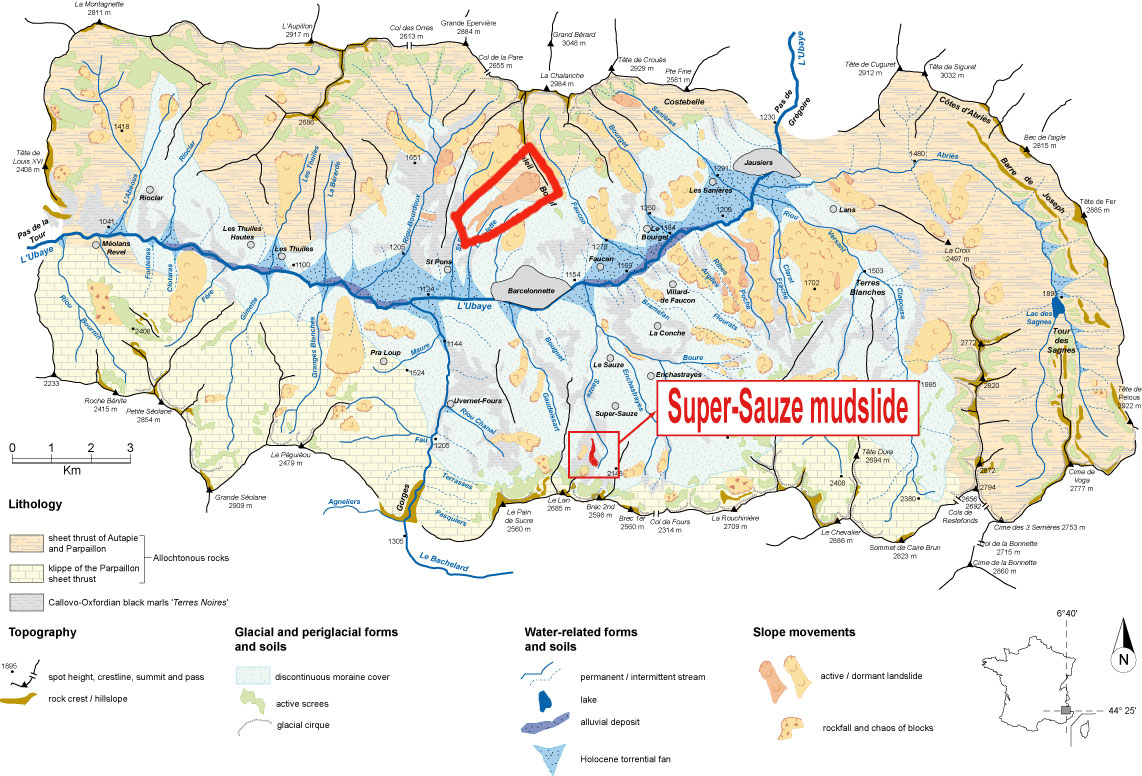
\includegraphics[width=0.6\linewidth]{carte_lavalette.png}
  \caption{Carte géologique des glissements de la zone d'Aiguilles. Au centre, dans le polygone en rouge, le glissement dormant de la Valette.}
\end{figure}


\begin{figure}[H]
  \centering
  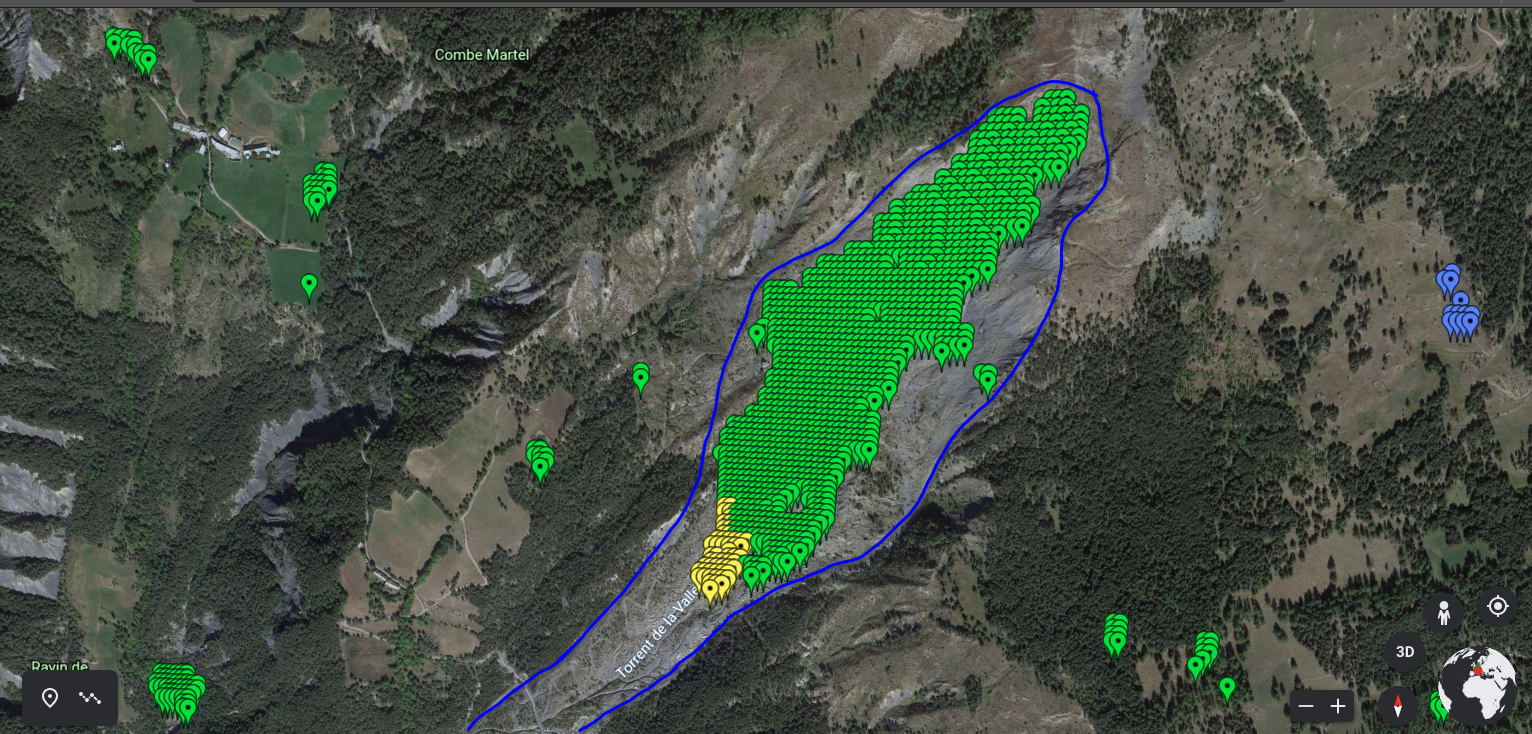
\includegraphics[width=0.6\linewidth]{first_landslide.png}
  \caption{Résultat du clustering temporel à l'aide de HDBSCAN visualisés dans Google Earth. Les marqueurs de même couleur représentent les pixels appartenant au même cluster. Les marqueurs en vert représentent le glissement de la Valette.}
\end{figure}

\section{Tâches à accomplir}
\begin{enumerate}
\item Améliorer le workflow de filtrage des pixels sans interêt pour pouvoir détecter les petits glissements de terrain;
\item Trouver une méthode pour quantifier la répartion spatiale des séries clusterisées afin de se passer de Google Earth;
\item Appliquer la décomposition en composantes independantes pour débruiter les signaux;
\item Fusionner le champ de déplacements de l'interférométrie radar et de l'imagerie optique;
\item Paralléliser les traitements.
\end{enumerate}
	
\end{document}





